\chapter{Venerdì 24/04/2020}
\section{Forme normali e normalizzazione}
\subsection{Forma normale di Boyce-Codd (BCNF)}
Uno schema, se rispetta questa forma normale, è privo di informazione duplicata. Una relazione $r$ è in forma normale di Boyce-Codd se per ogni dipendenza funzionale (non banale) $X \to Y$ definita su di essa, $X$ è superchiave di $r$. Questa forma normale richiede che i concetti in una relazione siano omogenei (cioè che tutte le proprietà siano direttamente associate alla chiave)
\paragraph{Presenza di dipendenze non banali} Se un insieme $F$ di dipendenze per $R$ non è in BCNF, allora in $F$ c'è almeno una dipendenza $X \to Y$ non banale con $X$ non superchiave di $R$.
\paragraph{Teorema} Dato uno schema $R$ e un insieme $F$ di dipendenze funzionali, se $F$ non contiene alcune $X \to Y$ non banale con $X$ non superchiave di $R$, allora neanche $F^+$ la contiene.
\paragraph{Metodo di verifica} Analizzo una ad una le dipendenze non banali in $F$ verificando se ognuna ha una superchiave come membro sinistro.
\begin{itemize}
	\item Occorre saper verificare se $F$ è minimale
	\item Occorre saper verificare se un insieme di attributi è superchiave di una relazione.
\end{itemize}
\paragraph{Come normalizziamo?} Se una relazione non è in BCNF la rimpiazziamo con altre relazioni BCNF: faccio questo decomponendo sulla base delle dipendenze funzionali, \underline{separando i concetti}.
\begin{center}
	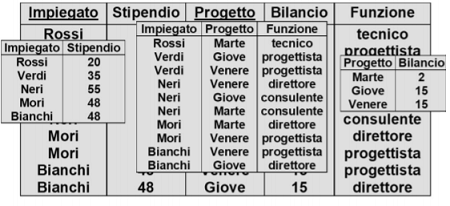
\includegraphics{images/142.PNG}
\end{center}
\paragraph{Esempio} Prendiamo la seguente tabella, che presenta certe dipendenze funzionali. 
\begin{center}
	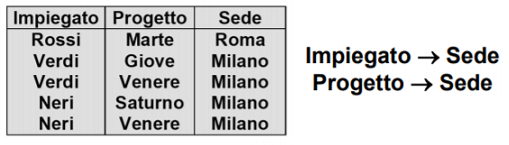
\includegraphics{images/143.PNG}
\end{center}
Procediamo alla decomposizione, ottenendo quanto segue
\begin{center}
	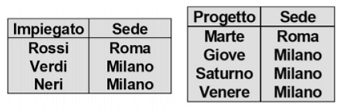
\includegraphics{images/144.PNG}
\end{center}
Un buon indicatore della correttezza di quanto stiamo facendo è la ricomposizione della tabella iniziale dopo aver effettuato le divisioni: se non posso riottenere la relazione iniziale allora qualcosa non va. Si individua che alcune composizioni di Boyce-Codd potrebbero presentare questo problema
\begin{center}
	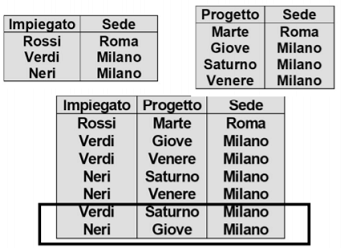
\includegraphics{images/145.PNG}
\end{center}
se io faccio JOIN con la sede ottengo tuple che precedentemente non esistevamo. Segue che dobbiamo trovare composizioni BCNF particolari!
\paragraph{Decomposizione senza perdita} Una istanza $r$ di una relazione $R$ si decompone senza perdita su $X_1$ e $X_2$ se il join naturale delle proiezione di $r$ su $X_1$ e $X_2$ è uguale ad $r$ stessa.
\paragraph{Algoritmo per la decomposizione in BCNF}  Assumiamo che tutte le dipendenze funzionali in $F$ abbiano un unico attributo come membro destro, e che $U$ sia l'insieme di tutti gli attributi di $R$.
\begin{itemize}
	\item $Decomponi(R,F)$
	\begin{itemize}
		\item Se esiste $X \to A$ in $F$ con $X$ non superchiave di $R$:
		\begin{itemize}
			\item Sostituisco $R$ con una relazione $R_1$ con attributi $U-A$ ed una relazione $R_2$ con attributi $X \cup A$
		\end{itemize}
		\item $Decomponi(R_1,F_{U-A})$
		\item $Decomponi(R_2,F_{X \cup A})$
	\end{itemize}
\end{itemize}
\paragraph{Esempio} Riprendiamo la solita tabella di prima. Abbiamo
\[F=\{Impiegato \to Sede, Progetto \to Sede \}\]
Applico l'algoritmo e ottengo
\[Decomponi(R,F)= R_1(Impiegato,Progetto), R_2(Impiegato, Sede)\]
\paragraph{Teorema, correttezza dell'algoritmo della decomposizione} Qualunque sia l'input, l'esecuzione dell'algoritmo su tale input termina e produce una decomposizione della relazione originaria tale che:
\begin{itemize}
	\item Ogni relazione ottenuta è in BCNF
	\item La decomposizione è senza perdita nel JOIN
\end{itemize}
\paragraph{Proiezione delle dipendenze funzionali di $R(U)$ su $X \subseteq U$} La proiezione di $F$ su $X$, denotata da $F_x$ è l'insieme delle dipendenze funzionali $Z \to Y$ in $F^+$ che coinvolgono solo attributi in $X$, cioè tali che $Z \subseteq X$ e $Y \subseteq X$.
\paragraph{Calcolare la proiezione delle DF su X}
\begin{itemize}
	\item CalcolaProiezione(F, X) :=
	\begin{itemize}
		\item Pongo $result = \{ \emptyset \}$
		\item Per ogni sottoinsieme proprio $S \subset X$, per ogni attributo $A \in X$ tale che $A \notin S$ e tale che non esiste alcun sottoinsieme $S'$ di $S$ tale che 
		\[S'\to A\]
		è in result, allora dico che se $A \subseteq S^{+}$ allora
		\[result=result \cup \{ S \to A \}\]
	\end{itemize}
\end{itemize}
Il metodo è funzionante ma in alcuni casi la proiezione di $F$ su $X$ può avere dimensione esponenziale rispetto alla dimensione di $F$ ed $X$. Si può dimostrare che nessun insieme equivalente a quello delle proiezioni non puiò avere cardinalità minore.
\paragraph{Esempio da internet per capire una spiegazione arzigogolata} Supponiamo di avere $R(A,B,C)$ e il seguente gruppo di dipendenze funzionali
\[F=\{ A\to B, B \to C, C \to A\}\]
individuo le seguenti proiezioni
\begin{itemize}
	\item $F_{AB}=\{ A \to B, B \to A\}$. 
	\item $F_{AC}=\{ A \to C, C \to A\}$
\end{itemize}
La prima proiezione è interessante perchè ci fa capire che non possiamo limitarci a verificare solo che $X \subseteq AB$ ed $Y \subseteq AB$ con $X \to Y$. Per comodità dobbiamo trovare, dato un insieme $F$, la sua copertura minimale. A quel punto dobbiamo stare attenti agli attributi sinistri, cioè controllare se essi non dipendono a loro volta dagli elementi su cui stiamo facendo la proiezione. In questo caso:
\begin{itemize}
	\item Pongo da $B \to C$ e $C \to A$
	\[BC \to A\]
	Ovviamente $C$ dipende da $B$ e per questo può essere rimosso.
	\item $BC$ è l'insieme $S$ che dicevamo nella spiegazione dell'algoritmo. In questo caso esiste un sottoinsieme $S'$ formato solo da $C$... Infatti possiamo dire che
	\[C \to A\]
\end{itemize}
\paragraph{Proprietà dell'algoritmo di decomposizione} A seconda dell'ordine con cui si considerano le dipendenze funzionali il risultato della decomposizione può cambiare. Riprendiamo l'esempio di prima e consideriamo le dipendenze funzionali in ordine diverso. Otteniamo uno schema diverso
\begin{verbatim}
	Rx(Impiegato, Sede)
	Ry(Impiegato, Progetto)
\end{verbatim}Supponiamo di voler inserire un nuovo impiegato, che sta a Milano, che lavorerà sul progetto Marte, con sede a Roma. 
\begin{center}
	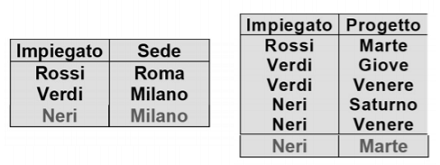
\includegraphics{images/150.PNG}
\end{center}L'inserimento è legittimo ma emerge un'inconsistenza relativa alla sede della persona e la sede del progetto
\begin{center}
	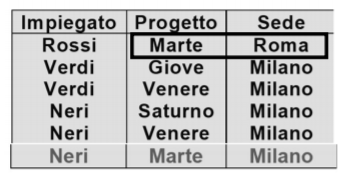
\includegraphics{images/146.PNG}
\end{center}
Non capiamo più se la sede indicata è quella dell'utente o del progetto! Non ho perdita di informazione attraverso il JOIN (le tuple che già esistevano prima della divisione della relazione esistono), ma la tupla nuova rappresenta qualcosa di inconsistente (la sede di Marte è a Milano, quando in realtà il progetto ha sede a Roma).  Segue che quanto detto ci garantisce il JOIN ma non le dipendenze (nell'esempio sono state perse).
\paragraph{Verifica di decomposizione senza perdita di dipendenze} La definizione di decomposizione senza perdita di dipendenze (considerando due relazioni $R1(X)$ ed $R2(Y)$ ottenute dalla decomposizione) è basata sul verificare che
\[(F_X \cup F_Y)^+=F^+\]
cioè la chiusura dell'insieme $F$ di dipendenze funzionali equivale alla chiusura dell'insieme ottenuto dall'unione della proiezione delle DF di $F$ su $X$ con la  proiezione delle DF di $F$ su $Y$. 
Per applicare questa definizione dobbiamo saper calcolare se un insieme di dipendenze funzionali è equivalente ad un altro. Inoltre dobbiamo saper calcolare la proiezione di un insieme di dipendenze funzionali su un insieme di attributi.
\paragraph{Qualità delle decomposizioni} Una decomposizione dovrebbe sempre garantire:
\begin{itemize}
	\item La BCNF
	\item L'assenza di perdite, in modo da poter ricostruire le informazioni originarie.
	\item La conservazione delle dipendenze, in modo da mantenere i vincoli di integrità originari.
\end{itemize}
\paragraph{Esempio di verifica della BCNF} Supponiamo che ogni dirigente abbia una sede e che ogni progetto possa essere diretto da più persone, ma in sedi diverse. In questo caso la chiave sarà \emph{Progetto Sede}.
\begin{center}
	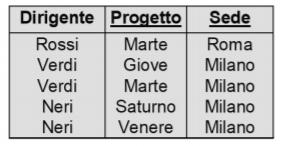
\includegraphics{images/151.PNG}
\end{center}
Il progetto da solo non può determinarmi il dirigente poichè questo può essere collocato in più sedi. Risulta valido dire che
\[Progetto\;Sede \to Dirigente\]
poichè ho un solo dirigente per ogni sede di progetto. Quanto segue, tuttavia, non è una BCNF
\[Dirigente \to Sede\]
poichè i dirigenti possono trovarsi in sedi diverse (Dirigente da solo non è chiave). Si osserva che la prima dipendenza coinvolge tutti gli attributi e che quindi decomporla comporta perderla!
\paragraph{Morale della favola} Risulta difficile trovare un BCNF che conservi le dipendenze e il JOIN insieme. Seguono ulteriori forme normali!

\subsection{Terza forma normale (3NF)}
Una relazione $r$ è in terza forma normale (3NF) se per ogni dipendenza funzionale non banale
\[X \to Y\]
definita su $r$, è verificata almeno una delle seguenti condizioni:
\begin{itemize}
	\item $X$ è superchiave di $r$
	\item Ogni attributo in $Y$ è contenuto in almeno una chiave di $r$
\end{itemize}
\begin{center}
	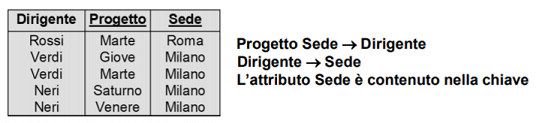
\includegraphics{images/183.PNG}
\end{center}
Si individua una ridondanza nella ripetizione della sede del dirigente per i vari progetti che dirige. 
\subsubsection{Confronto tra BCNF e 3NF}
\begin{itemize}
	\item La terza forma normale è meno restrittiva rispetto alla BCNF (ammette relazioni con alcune anomalie e ridondanze).
	\item Il problema di verificare se una relazione è 3NF è NP-completo (quindi il miglior algoritmo deterministico conosciuto ha complessità esponenziale nel caso peggiore).
	\item Tuttavia si ha un vantaggio: ottengo sempre una decomposizione senza perdite e con conservazione delle dipendenze.
\end{itemize}
\subsubsection{Algoritmo di decomposizione}
Nelle diapositive sono presentati due algoritmi di decomposizione:
\begin{itemize}
	\item Una che garantisce l'assenza di perdita sul JOIN e poi conserva le dipendenze
	\item Una che garantisce le dipendenze e poi risolve l'eventuale perdita sul JOIN
\end{itemize}

\begin{figure}[h]
	\begin{subfigure}{0.5\textwidth}
		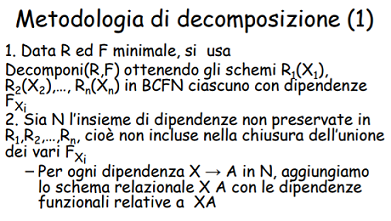
\includegraphics{images/184.PNG} 
		\caption{Primo metodo, utilizzato in \underline{tutti} gli esercizi della Prof}
	\end{subfigure}
	\begin{subfigure}{0.5\textwidth}
		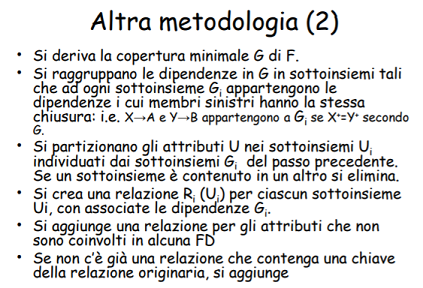
\includegraphics{images/185.PNG}
		\caption{Secondo metodo}
	\end{subfigure}
\end{figure}

Generalmente si verifica che lo schema 3NF sia anche BCNF. Se la relazione ha una sola chiave allora le due forme normali coincidono.
\section{Conclusioni}
Una decomposizione dovrebbe sempre garantire
\begin{itemize}
	\item BCNF o 3NF
	\item L'assenza di perdite (in modo da poter ricostruire le informazioni originarie)
	\item La conservazione delle dipendenze (in modo da mantenere i vincoli di integrità originari)
\end{itemize}
Il fatto che non si possa ottenere la BCNF è questione di cattiva progettazione. Tutta questa teoria serve per verificare la qualità dello schema logico: quanto spiegato può essere utilizzato anche nella progettazione concettuale per ottenere uno schema di buona qualità (verifica delle ridondanze, partizionamento di entità e relazioni....)


\section{Normalizzazione e progetto}

\subsection{Alcune definizioni aggiuntive}
\begin{itemize}
	\item Se in uno schema di relazione c'è più di una chiave, ognuna di esse è detta chiave candidata. Una delle chiavi è detta chiave primaria
	\item Un attributo di $R$ è detto attributo primo di $R$ se è membro di una qualche chiave candidata di $R$. Un attributo è detto non-primo se non è membro di alcuna chiave candidata
\end{itemize}
\subsection{Dipendenze funzionali complete e parziali}
\begin{itemize}
	\item \textbf{DF completa}: una DF $X \to Y$ si dice dipendenza funzionale completa (DFC) se la rimozione di qualsiasi attributo $A$ da $X$ comporta il venir meno della sussistenza della DF
	\item \textbf{DF parziale}: una DF $X \to Y$ si dice dipendenza funzionale parziale (DFP) se si possono rimuovere da $X$ certi attributi $A$ e la dipendenza continua a sussistere. Intendiamo che
	\[X-\{A\} \to Y\]
\end{itemize}
\subsection{Forme normali}
Il processo di normalizzazione sottopone uno schema di relazione a una serie di test per verificare se sono soddisfatte le proprietà tipiche di una forma normale. Individuiamo le seguenti forme:
\begin{itemize}
	\item Prima forma normale (1NF)
	\item Seconda forma normale (2NF)
	\item Terza forma normale (3NF)
	\item Forma normale di Boyce e Codd (BCNF)
	\item 4NF e 5NF (Non importante)
\end{itemize}
\subsubsection{Prima forma normale (1NF)}
La 1NF richiede che il dominio di un attributo comprenda solo valori atomici (semplici e indivisibili) e che il valore di qualsiasi attributo in una tupla sia un valore singolo del dominio. La forma normale 1NF è già parte integrante della definizione formale di relazione nel modello relazionale.

\subsubsection{Seconda forma normale (2NF)}
Uno schema di relazione $R$ è in forma 2NF se ogni attributo non-primo $A$ di $R$ è funzionalmente dipendente in modo completo da ogni chiave di $R$. Si osserva che possono esistere dipendenze tra attributi non-primi.

\subsubsection{Confronto tra forme normali}
La BCNF implica la 3NF\footnote{Se tutte le volte $X$ in $X\to Y$ è superchiave allora soddisfo tutte le volte una delle due condizioni possibili dalla 3NF}, che implica la 2NF. La 4NF e la 5NF riguardano dipendenza di tipo diverso, multivalore.